\section{Theorie}

\todo[inline]{Hier fehlt noch:

- etwas darüber was eine erfolgreiche automatisierung ausmacht. Faktoren über den

- Beispiele der Automatisierung aus der Literatur um die Forschungsfrage zu beantworten -> Hier der richtige Platz?}

\subsection{Forschungsstand}

% \todo[inline, color=igloo]{Vorschlag: Hier könntest Du mit dem Begriff "KI" beginnen und die Problematik ansprechen, dass zwar viele davon sprechen, aber (falls überhaupt) nur wenige wissen, was darunter zu verstehen ist. Vieles, was heute angeboten wird, basiert auf ML-Ansätzen, wie z.B. und dann kannst Du best practices aufweisen.}

Die künstliche Intelligenz ist ein sehr aktuelles und deshalb auch in der Literatur oft diskutiertes Themengebiet. Bereits 2009 geben \textcite{Russell2009} auf über 1000 Seiten einen noch immer aktuellen und sehr umfangreichen Überblick über das Themengebiet. Weiter vertiefen die beiden Autoren viele Teilgebiete der künstlichen Intelligenz und erläutern Grundlegende Konzepte ausführlich.

% Einen etwas mathematischeren Überblick über das Thema künstliche Intelligenz geben \textcite{Goodfellow2016}. Die Diskussion reicht von den absoluten Grundlagen, der linearen Algebra, bis hin zu Deep Generative Models, eine fortgeschrittene Anwendung der künstlichen Intelligenz~\autocite{Goodfellow2016}.

Es kann gesagt werden, dass in der Grundlagenforschung zur künstlichen Intelligenz bereits viele Forschungsergebnisse vorliegen. Es werden etliche, etablierte und experimentelle, Techniken diskutiert und täglich weiterentwickelt. Zur Automatisierung eines Geschäftsprozesses und somit für die Entwicklung eines Prototypen für die AXA Gesundheitsvorsorge stehen viele Möglichkeiten zur Verfügung.

Um einen ersten Überblick über das Themengebiet zu erhalten, werden einige Techniken im Bereich der künstlichen Intelligenz, welche für die Beantwortung der Forschungsfrage sowie für die Entwicklung des Prototypen relevant sind, in den folgenden Kapiteln erläutert.

\subsubsection{Natural Language Processing}

Natural Language Processing (kurz NLP) beschreibt das Gebiet der Forschung und Anwendung von Computern um natürliche Sprache, in Wort und Schrift, zu verstehen und verarbeiten. NLP umfasst diverse Forschungsfelder wie beispielsweise die maschinelle Übersetzung, die Spracherkennung sowie die Informationsextraktion~\autocite{Chowdhury2003}. 

Für diese Arbeit ist das Themengebiet des Natural Language Processing insofern relevant, als dass es die Grundlage für die Verarbeitung von Rechnungen bildet. Mit Techniken aus diesem Gebiet werden die Inhalte der Rechnungen vom Computer verstanden und verarbeitet.

\subsubsection{Neuronale Netzwerke}

Abgesehen von Rechenaufgaben sind Menschen Leistungsfähiger als Computer. Wir sind beispielsweise in der Lage, Gesichter zu erkennen oder in einem dunklen Raum Personen anhand Ihrer Stimme zu identifizieren. Der interessanteste Unterschied des Menschlichen Gehirns zu einem Computer ist allerdings der Fakt, dass unser Gehirn lernt ohne ein Software-Update zu erhalten. Wir brauchen nicht erst eine neue Software um das Fahrradfahren zu erlernen. Doch wie funktioniert das~\autocite{Krogh2008}?

Die Berechnungen unseres Gehirn werden durch hoch vernetzte Neuronen gemacht. Dabei interagieren die Neuronen mit Stromimpulsen durch die Neuronale Verkabelung, bestehend aus Nervensäulen, Synapsen und Zellfortsätzen. 1943 Modellierten McCulloch und Pitts Neuronen als Schalter, welche aufgrund der eingehenden Signale Ein- oder Ausgeschaltet sind. Die Gewichtung der eingehenden Signale waren dabei die Synapsen. Aus diesem Modell entstand das Konzept von Neuronalen Netzwerken~\autocite{Krogh2008}.

Damit ein Neuronales Netzwerk Leistungsfähig werden kann, muss es ähnlich wie ein Mensch, erst lernen. Das computersimulierte Lernen, auch Machine Learning genannt, funktioniert dabei so, dass für die Gewichte der Verbindungen, sprich die stärke der Synpasen, ein zufälliger Wert gewählt wird. Anschliessend wird eine Beispielaufgabe vom Netzwerk gelöst. Das Resultat des Netzwerks ist zu Beginn höchstwahrscheinlich falsch und die Gewichte im Netzwerk werden mit einem kleinen Schritt angepasst. Es werden dann immer weitere Beispielaufgaben gelöst und die Gewichte entsprechend angepasst bis das Netzwerk die gewünschten Resultate liefert~\autocite{Krogh2008}.

Seit mehreren Jahren liefern Neuronale Netzwerke bessere Resultate als klassische Techniken. Dabei werden Neuronale Netzwerk vorwiegend für visuelle Aufgaben und immer häufiger auch zur Verarbeitung Natürlicher Sprache verwendet~\autocite{Olah2014b}.

% \todo[inline]{Say a word on overfitting}

% \todo[inline]{Say something about learning strategies (supervised / unsupervised)}

\subsubsection{Long-Short-Term-Memory Netzwerke}

Menschen starten ihren Denkprozess nicht jede Sekunde von neuem. Beim Lesen wird jedes Wort aufgrund des Verständnisses des vorherigen Wortes verstanden. Gedanken sind persistent. Genau solche persistenten Gedanken sind mit dem bisherigen Ansätzen für Neuronale Netze nicht modellierbar. Hier kommen Recurrent Neural Networks (kurz RNN) ins Spiel. Recurrent Neural Networks sind Neuronale Netzwerke mit integrierten Schlaufen~\autocite{Olah2015}. 

In Abbildung \ref{rnn1} wird ein RNN mit einer Schlaufe dargestellt. Daneben ist das selbe Netzwerk in einer anderen, ausgerollten Weise zu sehen. Die Abbildung verdeutlicht, wie Informationen von einem Neuron zum anderen fliessen können. Mit diesem Informationsfluss von Neuron zu Neuron werden die Resultate jeweils von den vorhergehenden Neuronen beeinflusst. Damit wird eine Art Kurzzeitgedächtnis geschaffen, welches dem Neuronalen Netzwerk erlaubt mit Kontextinformationen zu arbeiten~\autocite{Olah2015}.
\begin{figure}[h]
    \captionsetup{width=.8\linewidth}
    \caption{Infromationsfluss durch ein Recurrent Neural Network dargestellt als Schlaufe (links) und als Sequenz (rechts)}
    \label{rnn1}
    \centering
    \vspace{0.2cm}
    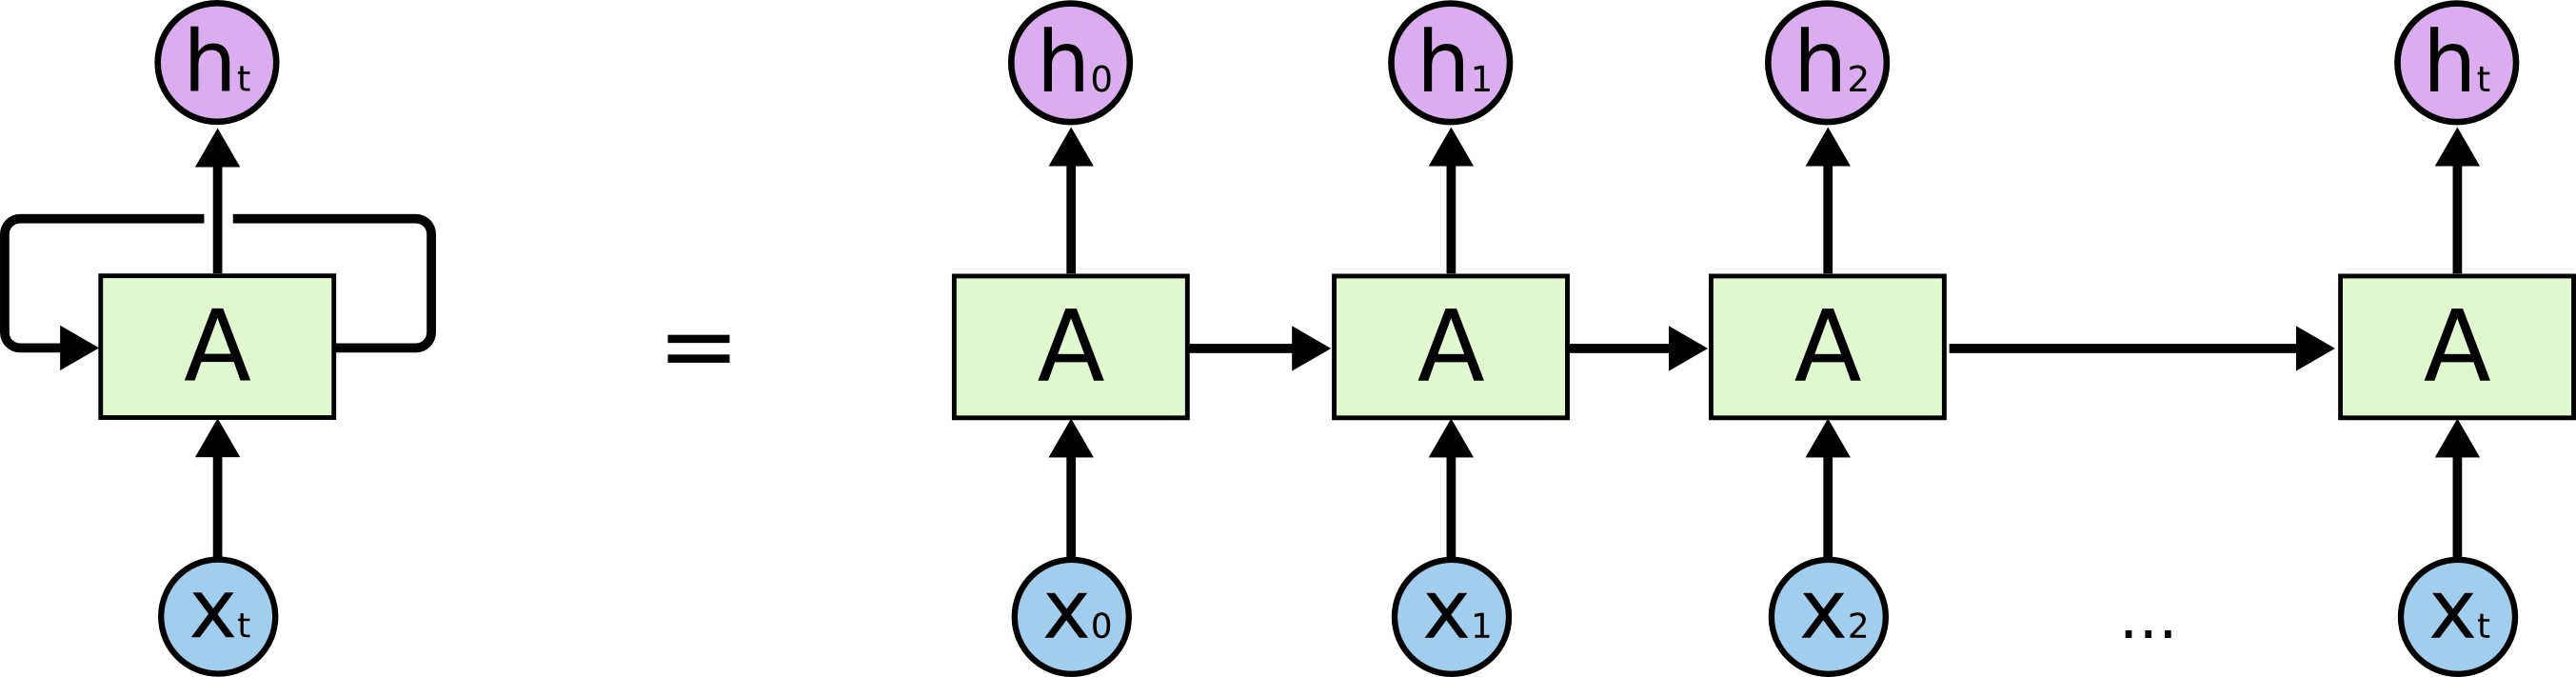
\includegraphics[width=0.6\textwidth]{graphics/rnn1.png}\\
    \vspace{0.3cm}
    \caption*{Quelle: \textcite{Olah2015}}
\end{figure}

Ein Problem von RNNs ist, dass nur ein Kurzzeitgedächtnis zur Verfügung steht. Liegen Informationen etwas länger zurück, sprich der Abstand zwischen den beiden relevanten Neuronen ist zu gross, gehen diese Informationen verloren. Eine Lösung für diese Problematik bieten Long-Short-Term-Memory (kurz LSTM) Netzwerke. Diese Spezialform von Recurrent Neural Networks arbeitet mit sogenannten Gates, um zu regulieren, wie viel Kontextinformationen behalten oder vergessen werden sollen. Mit vier solchen Gates, bestehend aus einem Neural Network Layer und einer Pointwise Operation (vgl. Abbilung \ref{lstm1}), ist ein LSTM Netzwerk in der Lage, nicht nur ein Kurz- sondern auch ein Langzeitgedächtnis aufzubauen~\autocite{Olah2015}.
\begin{figure}[h]
    \captionsetup{width=.8\linewidth}
    \caption{Veranschaulichung des Informationsflusses eines LSTM Netzwerk mit seinen vier internen Schichten}
    \label{lstm1}
    \centering
    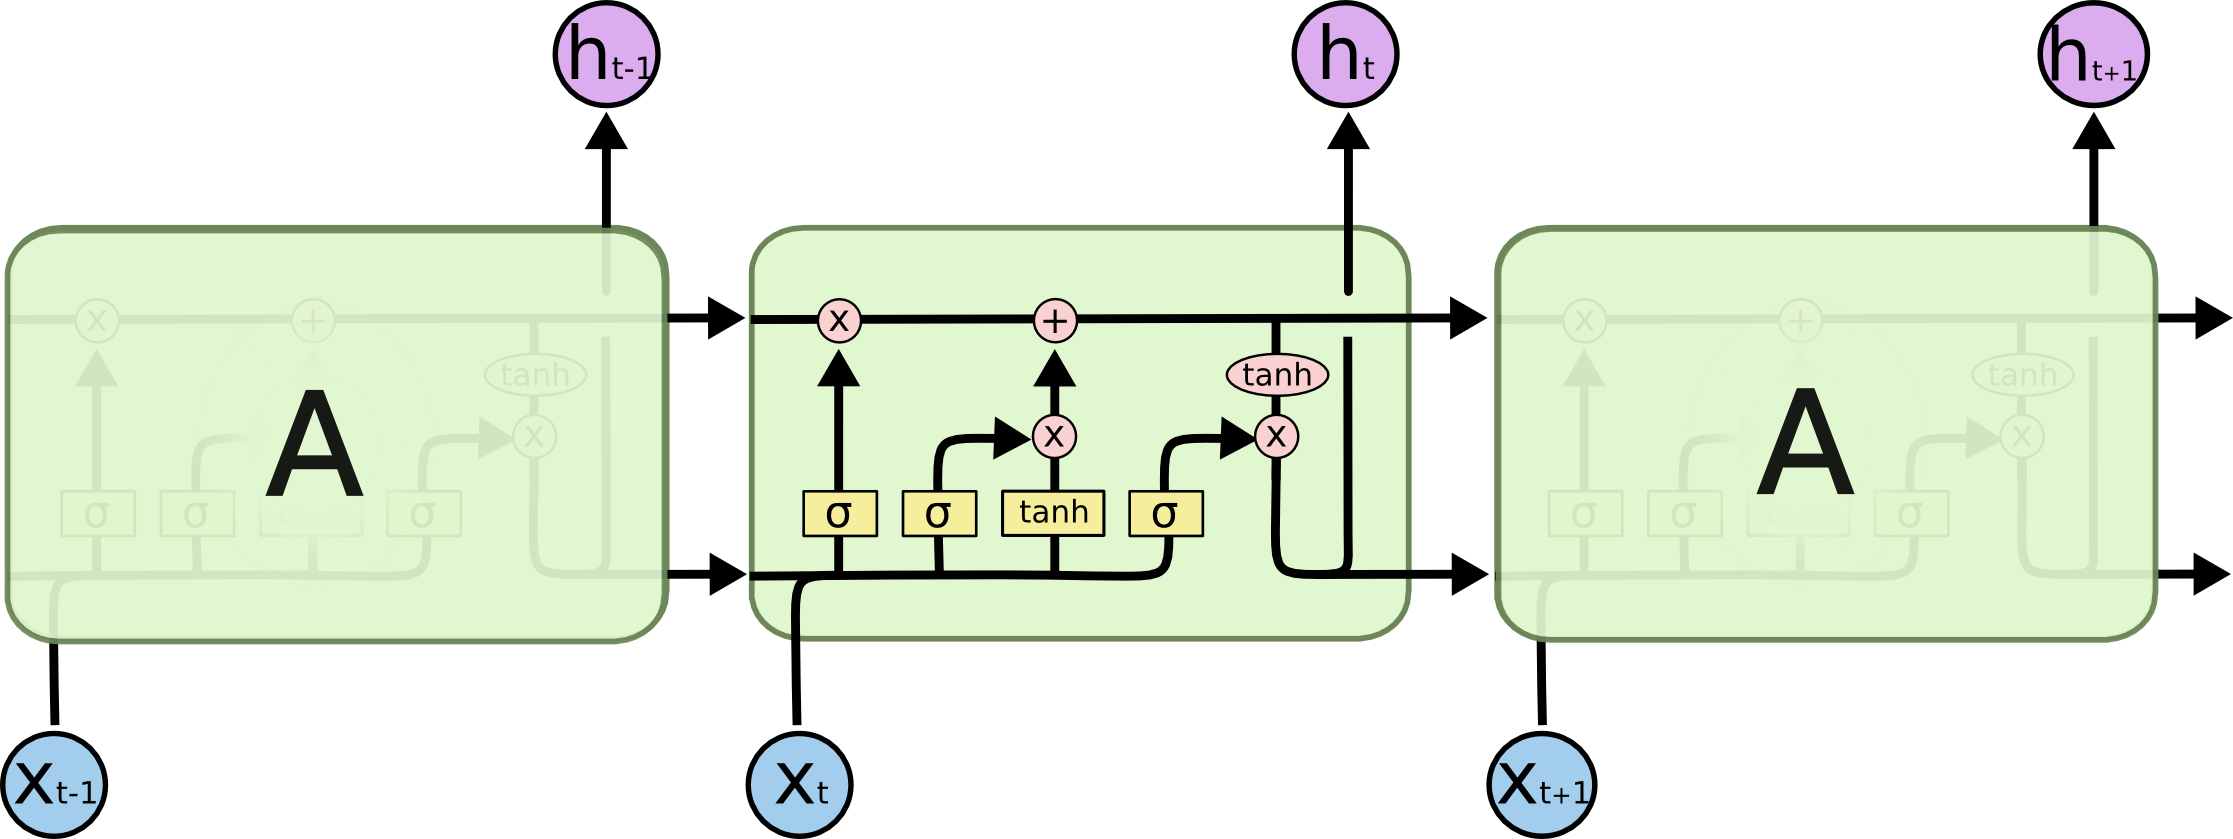
\includegraphics[width=0.6\textwidth]{graphics/lstm.png}\\
    \vspace{0.5cm}
    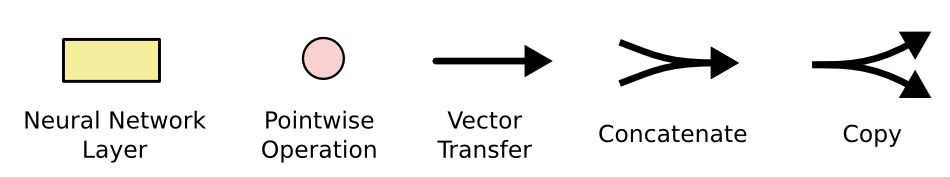
\includegraphics[width=0.6\textwidth]{graphics/lstm-notation.png}\\
    \vspace{0.1cm}
    \caption*{Quelle: \textcite{Olah2015}}
\end{figure}

Recurrent Neural Networks wurden in der Vergangenheit sehr erfolgreich für viele Aufgaben, wie beispielsweise die Spracherkennung, Sprachmodellierung, maschinelle Übersetzung sowie Bilderkennung, angewendet. In den meisten Fällen wurden dabei LSTM Netzwerke angewendet, da die Resultate um ein Vielfaches besser ausfallen als mit herkömmlichen RNNs~\autocite{Olah2015}.

LSTM Netzwerke sind für diese Arbeit besonders zur Texterkennung und Rechtschreibkorrektur interessant. Diese beiden Techniken werden im Prototypen der Rechnungsindexierung verwendet.

\subsubsection{Texterkennung}

Ein wichtiger Bestandteil des Prototypen zur Indexierung von Rechnungen ist die Erkennung von Texten, ob Druckbuchstaben oder Handschrift, auf den Rechnungen. Die erkannten Texte bilden die Grundlage für jegliche digitale Verarbeitung der Rechnungen.

Die herkömmliche Feature-detection in Texterkennungssoftware wird immer mehr mit künstlicher Intelligenz ersetzt. \textcite{Neuberg2017} beschreibt wie Dropbox künstliche Intelligenz anwendet, um Texte aus Fotografien von Dokumenten durchsuchbar zu machen. Zur Anwendung kommen dabei verschiedene Techniken aus dem Bereich der künstlichen Intelligenz: \textit{Convolutional Neural Network}\footnote{Ein Convolutional Neural Network ist eine Spezialform eines Neuronalen Netzwerks bei welchen, etwas vereinfacht ausgedrückt, viele Kopien des gleichen Neurons zum Einsatz kommen\autocite{Olah2014}.} (CNNs),  \textit{Long-Short-Term-Memory} (LSTM) Netzwerke, \textit{Connectionist Temporal Classification}\footnote{CTC ist ein Konzept aus dem Training von Neuronalen Netzwerken, welches vor allem in der Handschrifterkennung Verwendung findet. Dabei wird eine spezielle Trainingsfunktion verwendet, durch welche die Positionierung von Buchstaben generalisiert und somit der Lernprozess des Neuronalen Netzwerks vereinfacht werden kann~\autocite{Scheidl2018}} (CTC) und weitere~\autocite{Neuberg2017}.

Auch die Texterkennungssoftware Tesseract, welche ursprünglich als PhD Forschungsprojekt im HP Lab entwickelt wurde und seit 2005 als Open Source Software zur freien Verfügung steht, verwendet seit Version 4 künstliche Intelligenz~\autocite{Smith2007}. So wurde die Feature-detecion durch ein LSTM Netzwerk mit mehr als 100 Schichten ersetzt. Die Texterkennung konnte so nicht nur Qualitativ stark verbessert werden sondern ist auch einiges schneller als zuvor. Doch auch nach den Verbesserungen sind die Ergebnisse nicht perfekt und müssen fallspezifisch optimiert werden~\autocite{O.V.2018, O.V.2018a}.

\subsubsection{Word embedding}

Neuronale Netzwerke funktionieren mit Zahlen. Damit auch Wörter und ganze Sätze von solchen Netzwerken verarbeitet werden können, muss eine geeignete Repräsentation von Wörtern durch Zahlen gefunden werden. Der Prozess, mit welchem ein Wort in eine zahlen-basierte Repräsentation gebracht wird, nennt sicht Word embedding~\autocite{Olah2014b}.

Die ersten Word embeddings wurden von \textcite{Bengio2001} eingeführt. Trotz des schon fortgeschrittenen Alter dieses Forschungsgebiet ist es noch immer hoch interessant und in voller Fahrt~\autocite{Olah2014b}.

\begin{wrapfigure}{r}{0.5\textwidth} 
    \caption{Modulares Netzwerk zur Validierung von 5-Grammen mit einer Word embedding Funktion ($W$) und einem Neuronalen Netzwerk ($R$)}
    \label{wordembeddingtraining}
    \centering
    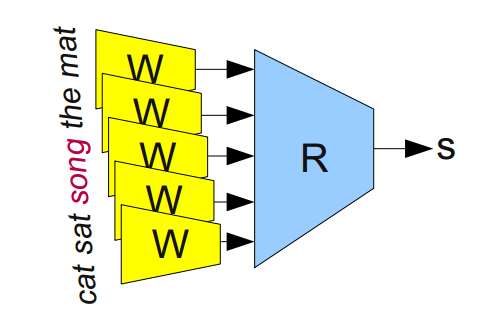
\includegraphics[width=0.48\textwidth]{graphics/wordembeddingtraining.png}
    \caption*{Quelle: \textcite{Olah2014b}}
\end{wrapfigure}
Technisch gesehen ist ein Word embedding eine parametrierte Funktion, welche Wörter einer bestimmten Sprache in einen hoch-dimensionalen Vektor (typischerweise 200-500 Dimensionen) transformiert. Um diese hoch komplexe Funktion zu definieren, kommt, wie bei den Neuronalen Netzwerken, Machine Learning zum Einsatz. \textcite{Olah2014b} beschreibt in seinem Artikel ein Beispiel, bei welchem eine solche Word embedding Funktion trainiert wird, indem die Resultate aus dem Word embedding in ein Neuronales Netzwerk zur Prüfung eines 5-Grammes gespiesen werden und dann das Gesamtkonstrukt trainiert wird (vgl. Abbildung \ref{wordembeddingtraining})~\autocite{Olah2014b}.

Um sich Word embeddings besser vorstellen zu können, zieht \textcite{Olah2014b} zwei verschiedene Möglichkeiten der Visualisierung heran.

Die erste Visualisierung bedient sich dem t-SNE Algorithmus um die hoch-dimensionalen Vektoren in einem zweidimensionalen Diagramm darzustellen. In diesem Diagramm ist klar zu erkennen, dass ähnliche Wörter nahe zusammen sind (vgl. Abbildung \ref{wordembeddingtsne})~\autocite{Olah2014b}.
\begin{figure}[h]
    \centering
    \caption{t-SNE Darstellung eines Word embeddings, die verdeutlicht, dass ähnliche Wörter ähnliche Vekotren aufweisen}
    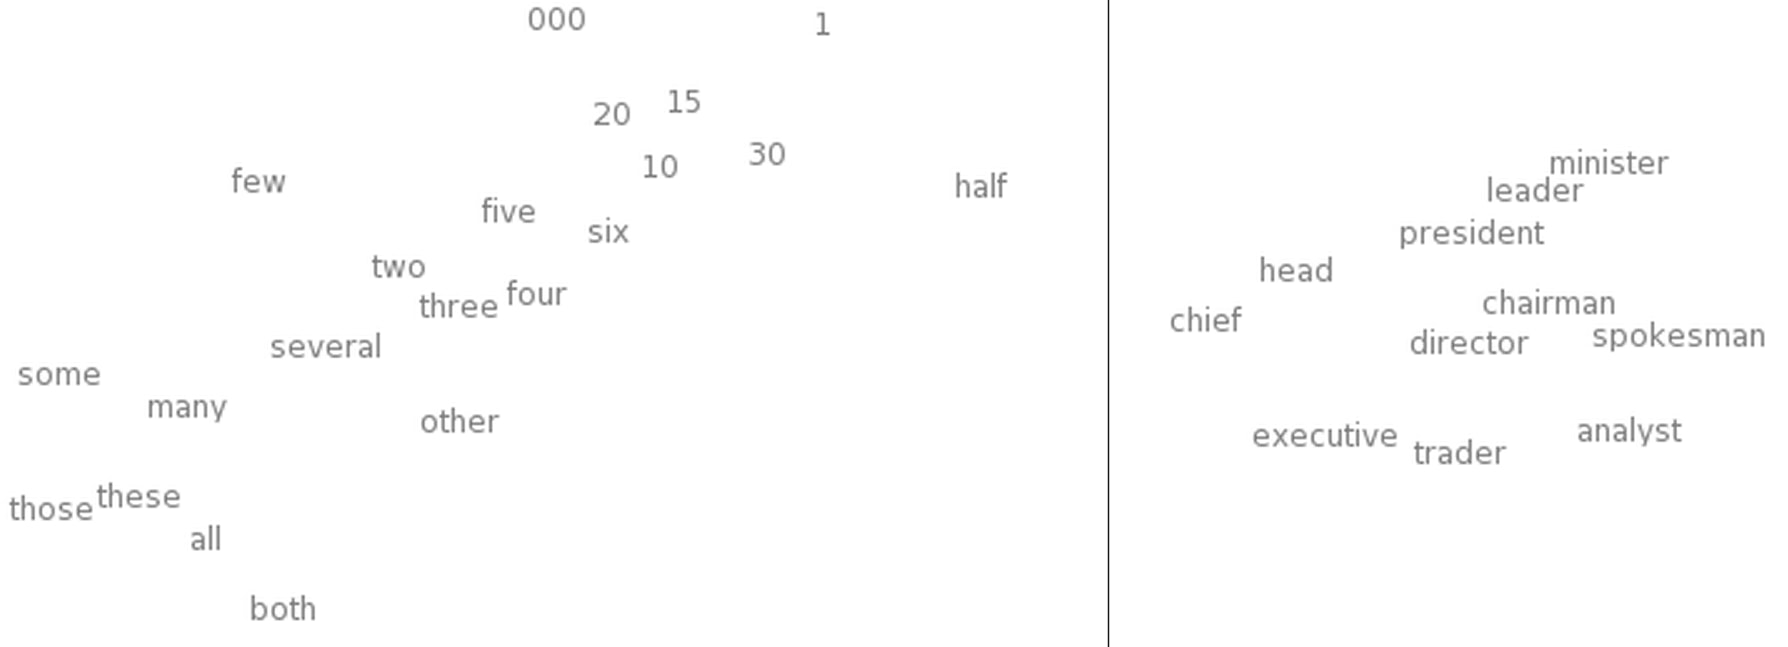
\includegraphics[width=\textwidth]{graphics/wordmebeddingtsne.jpg}
    \caption*{Quelle: \textcite{Turian2010} in \textcite{Olah2014b}}
    \label{wordembeddingtsne}
\end{figure}

Die zweite Visualisierung listet in einer Tabelle (vgl. Tabelle \ref{wordembeddingtable}) für sechs Wörter die nächsten Embeddings, sprich mit den mathematisch nächsten Vektoren, auf. So werden beispielsweise unter dem Titel \textit{FRANCE} neben \textit{EUROPA} diverse weitere Länder aufgelistet.
\begin{table}[h]
\centering
    \caption{Sechs Ausgangswörter mit den ihnen ähnlichsten Word embeddings, sprich mit den mathematisch nächsten Vektoren}
    \label{wordembeddingtable}
    \renewcommand{\arraystretch}{1.25}
    \setlength{\tabcolsep}{3pt}
    \small
    \begin{tabular}{ | l | l | l | l | l | l |}
    \hline
    \rowcolor{ccc} FRANCE & JESUS & XBOX & REDDISH & SCRATCHED & MEGABITS \\ \hline
    AUSTRIA & GOD & AMIGA & GREENISH & NAILED & OCTETS \\ \hline
    BELGIUM & SATI & PLAYSTATION & BLUISH & SMASHED & MB/S \\ \hline
    GERMNAY& CHRIST & MSX & PINKISH & PUNCHED & BIT/S \\ \hline
    ITALY & SATAN & IPOD & PRUPLISH & POPPED & BAUD \\ \hline
    GREECE & KALI & SEGA & BROWNISH & CRIMPED & CARATS \\ \hline
    SWEDEN & INDRA & PS\textit{NUMBER} & GREYISH & SCRAPED & KBIT/S \\ \hline
    NORWAY & VISHNU & HD & GRAYISH & SCREWED & MEGAHERTZ \\ \hline
    EUROPE & ANANDA & DRAMCAST & WHITISH & SECTIONED & MEGAPIXELS \\ \hline
    HUNGARY & PARVATI & GEFORCE & SILVERY & SLASHED & GBIT/S \\ \hline
    SWITZERLAND & GRACE & CAPCOM & YELLOWISH & RIPPED & AMPERES \\ \hline
    \end{tabular}
    \caption*{Quelle: \textcite{Collobert2011} in \textcite{Olah2014b}}
\end{table}

Sowohl Abbildung \ref{wordembeddingtsne} als auch Tabelle \ref{wordembeddingtable}, zeigen die Stärke von Word embeddings auf: Ähnliche Wörter werden mit ähnlichen Vektoren versehen und so wird eine komplexe Landschaft von Zusammengehörigen Wörtern gebildet. Aufgrund dieser Eigenschaft verändert sich durch den Austausch eines Wortes mit einem Synonym der Input-Vektor für ein nachfolgendes Neuronales Netzwerk nur geringfügig, da die Word embeddings der beiden Synonyme sehr ähnlich sind. Somit muss dieses nachfolgende Neuronale Netzwerk nicht für alle Wörter der Welt trainiert werden, sondern kann auf die Generalisierung durch das Word embedding aufbauen~\autocite{Olah2014b}.

Word embeddings sind zu einem extrem wichtigen Baustein bei der Verarbeitung von Natürlichen Texten geworden. Neben Input und Output Repräsentationen bei NLP Tasks können Word embeddings auch Output Repräsentationen in der Bilderkennung sein~\autocite{Olah2014b}. 

Für den Prototypen bilden Word embeddings eine wichtige Grundlage, da durch diese Technik die in den Rechnungen enthaltenen Wröter und Sätze in eine generalisierte, durch Neuronale Netzwerke verarbeitbare Form gebracht werden können.

\subsubsection{Korrektur von Rechtschreibung und Grammatik}

Trotz grossem Fortschritt, nicht zuletzt dank der Verwendung von künstlicher Intelligenz, im Bereich der Texterkennung, werden Texte nicht zu 100\% korrekt erkannt. So schleichen sich falsch erkannte Buchstaben ein, welche nicht nur Wörter sondern auch ganze Sätze bedeutungslos machen. Um solche Fehler zu korrigieren, wird auf die Rechtschreibung- und Grammatik-Korrektur zurückgegriffen. Während diverse Korrekturprogramme regelbasierte Software anwenden, wurde auch in diesem Bereich bereits erfolgreich künstliche Intelligenz angewandt.

Mit Hilfe der in einem vorherigen Kapiteln eingeführten Technik des Word embeddings und von LSTM Netzwerken lässt sich diese Problematik angehen. So kann ein Modulares Netzwerk aus Word embeddings und mehreren LSTM Schichten verwendet werden, um eine Rechtschreibkorrektur vorzunehmen. So beschreibt \textcite{Weiss2016} in seinem Blog, wie mit einem einfachen Neuronalen Netzwerk, bestehend aus nur 4 LSTM und 4 Dropout Schichten, bereits erfolgreich Rechtschreibfehler korrigiert werden können. 

% can't use wrapfigure here as otherwise the next sections wraps too
\begin{figure} % wrapfigure}{l}{0.5\textwidth}
    \centering
    \caption{Vergleich der Erfolgsrate bei der Prüfung von 418 Textsnippets}
    \label{deepgrammar}
    \begin{tikzpicture}
        \begin{axis}[
            ytick={0,10,20,30,40,50,60,70},
            ymin=0,
            ymax=70,
            xticklabels=\empty,
            xtick style={draw=none},
        	ylabel={Erfolgsrate [\%]},
        	enlargelimits=0.05,
        	ybar={10pt},
            bar width=20pt,
            legend style={cells={anchor=west},at={(1,-0.02)}, legend columns=2}, 
            area legend,
        ]
            \addplot[fill=cChart1]
            	coordinates {(0,61)};
            \addplot[fill=cChart2]
            	coordinates {(0,54)};
            \addplot[fill=cChart3]
            	coordinates {(0,54)};
            \addplot[fill=cChart4]
            	coordinates {(0,65)};
            \addplot[fill=cChart5]
            	coordinates {(0, 58)};
            \legend{Word,Grammarly,Google,LanguageTool,Deepgrammar}
        \end{axis}
    \end{tikzpicture}
    \caption*{Quelle: In Anlehnung an \textcite{Mugan}}
\end{figure} %wrapfigure}
Nicht nur zur Korrektur von Rechtschreibfehler ist ein Neuronales Netzwerk anwendbar. So kann unter deepgrammar.com ein Experiment gefunden werden, bei welchem ein solches Netzwerk zur Grammatikprüfung angewendet wird. Die Resultate, welche in der Tabelle \ref{deepgrammar} zu sehen sind, sind erstaunlich. Obwohl DeepGrammar erst seit einem Jahr existiert und dabei von nur einer Person entwickelt wurde, funktioniert das Netzwerk beinahe so gut wie \textit{Microsoft Word}\footnote{Microsoft Word ist ein Programm zur Textverarbeitung und Dokumenterstellung von Microsoft~\autocite{MicrosoftCorporation2018}.} oder \textit{Language Tool 3.1}\footnote{\enquote{LanguageTool ist eine Software zur Textprüfung [...]}~\autocite{LanguageTool2018}} und sogar besser als \textit{Grammarly}\footnote{Grammarly verspricht präzise, kontextabhängige Korrekturen von Texten~\autocite{GramarlyInc.2018}} und \textit{Google Docs}\footnote{Google Docs ist eine Online-Lösung zur Textverarbeitung von Google~\autocite{GoogleLLC2018}}~\autocite{Mugan}.

% TODO: Mugan erwähnt eine bessere Studie. In der Thesis diese verwenden, da Zahlen aus DeepGrammar nicht 100% korrekt sind https://arxiv.org/pdf/1807.01270.pdf

Ein weiterer grosser Vorteil von Neuronalen Netzwerken zur Fehlerkorrektur erwähnt \textcite{Mugan2018} in einer persönlichen Kommunikation: Das Neuronale Netzwerk kann auf das Domänenspezifische Lexikon trainiert werden. Das Netzwerk kann beispielsweise mit medizinischen Begriffen aus den Rechnungen trainiert werden, so dass die Resultate des in dieser Arbeit entwickelten Prototypen noch besser werden~\autocite{Mugan2018}.

\subsubsection{Informationsextraktion aus natürlichen Texten}

% https://en.wikipedia.org/wiki/Named-entity_recognition
% https://en.wikipedia.org/wiki/Medical_classification

Informationsextraktion beschreibt das Themengebiet rund um die Extraktion von strukturierten Informationen aus unstrukturiertem oder halb-strukturiertem Text. In diesem Kapitel werden einige Techniken aus diesem Themengebiet kurz erläutert und deren Ein\-satz\-mög\-lich\-keit für die Entwicklung des Prototypen diskutiert.

Eine \textit{Regular Expression} (kurz RegEx) ist ein Ausdruck, welcher eine Zeichenkette beschreibt. Diese Ausdrücke funktionieren ähnlich wie arithmetische Ausdrücke: Es werden Operatoren verwendet, um mehrere Ausdrücke zu einem komplexeren Ausdruck zusammenzufassen\autocite{Xiao2004}.

\textcite{Xiao2004} beschreibt als einfaches Beispiel den Ausdruck \texttt{[a,p]m [0-9]+:[0-9]+} um Zeitangaben wie AM 12:45 zu extrahieren. Dieses Beispiel zeigt einerseits die Einfachheit dieser Technik aber auch die Grenzen. 12:45 AM wird beispielsweise nicht erkannt, da AM hier nach anstelle vor der Uhrzeit steht. 

Ein weiterer Nachteil von Regular Expressions ist, dass Kontextinformationen nicht be\-rück\-sich\-tigt werden. Folgendes Beispiel von \textcite{Xiao2004} zeigt dies auf: Der Ausdruck \texttt{[0-9]+} ist zwar in der Lage aus dem Text \texttt{100\$} die Zahl \texttt{100} zu extrahieren, allerdings geht die Information, dass es sich hier um einen Geldbetrag handelt, verloren.

Um eine hohe Präzision bei der Informationsextraktion zu ermöglichen, sollten Regular Expressions also nur mit Vorsicht und in Kombination mit anderen Techniken verwendet werden~\autocite{Xiao2004};

Trotz der Nachteile der Regular Expressions können diese in der Entwicklung des Prototypen hilfreich sein. In Rechnungen werden viele Beträge, Daten und ähnliche Ausdrücke verwendet, welche mit Regular Expressions erkannt werden können.

\textit{Named Entity Recognition and Classification} (kurz NERC oder NER), beschreibt das erkennen und kategorisieren von Entitäten, sprich Wörter oder Wortgruppen aus natürlichen Texten~\autocite{Nadeau2007}.

Der Begriff \textit{Named Entity} wurde bei der Formulierung der Aufgabenstellung der sechsten Message Understanding Conference im Jahre 1995 definiert~\autocite{Borthwick1998}. So wurde bereits damals erkannt, dass die Extraktion von Namen, von Personen, Organisationen oder Lokationen, nummerischen Ausdrücken, Daten und Prozent-Ausdrücken wichtig ist~\autocite{Nadeau2007}.

Für die Named Entity Recognition and Classification stehen einige freie Softwarelösungen zur Verfügung. So veröffentlicht beispielsweise Stanford eine Java Implementierung und SpaCy, eine Sammlung von Natural Language Processing Software, beinhaltet eine Implementierung in Python~\autocite{StanfordNLPGroup, ExplosionAI}.

Die Anwendung von NERC ist für das Fallbeispiel äusserst Interessant. Die Erkennung von Namen von Personen ist hilfreich zur Erkennung des Patienten und des Leistungserbringers. Weiter hilft die Erkennung von Daten der Ermittlung des Behandlungsdatums und nicht zuletzt kann durch die Erkennung und Klassifizierung von nummerischen Ausdrücken der Gesamtbetrag sowie die Beträge einzelner Positionen ermittelt werden.

Die letzte Technik welche in diesem Kapitel erläutert wird, ist das \textit{Part of Speech Tagging} (kurz PoS-Tagging). Beim PoS-Tagging werden Wörter und Satzzeichen ihren Wortarten (Nomen, Adjektive, etc.) zugewiesen~\autocite{Xiao2004}.

Die grösste Herausforderung beim PoS-Tagging sind Wörter welche verschiedenen Wortgruppen zugewiesen werden könnten. Beispielsweise kann das Wort \textit{widerwillig} im Satz \textit{Sie nannten den Täter widerwillig.} als Adjektiv oder Adverb aufgefasst werden und somit die Bedeutung des Satzes vollkommen verändern~\autocite{Volk}.

% Es gibt diverse Arten von Implementierung des PoS-Tagging, welche in regelbasierte, stochastische und neuronale Verfahren unterteilt werden können. Ein weit verbreiteter Ansatz ist die Verwendung von Hidden Markov Modellen. Ein Hidden Markov Modell ist ein stochastisches Modell, welches Zustände mit übergangswahrscheinlichkeiten modelliert.

Die Verwendung von PoS-Tagging kann bei Rechnungen mit einem Prosatext von Vorteil sein. Wie viele relevante Informationen in Prosatexten von Rechnungen verborgen sind, muss sich aber erst noch zeigen.

Die beschriebenen Techniken bieten eine gute Grundlage um damit eine erste Implementierung eines Prototypen zur Rechnungsindexierung zu beginnen. vcd

\subsection{Künstliche Intelligenz in der Automatisierung von Geschäftsprozessen}

Anwendungsbeispiele aus der Literatur
Wo wird was bereits erfolgreich gemacht, welche Methoden/Praktiken werden eingesetzt?